\documentclass[11pt,a4paper]{article}

\usepackage[utf8]{inputenc}
\usepackage[T1]{fontenc}
\usepackage[spanish,es-noshorthands]{babel}
\addto\captionsspanish{\renewcommand{\tablename}{Tabla}}
\usepackage{lmodern}
\usepackage[margin=2.3cm]{geometry}
\usepackage{amsmath}
\usepackage{graphicx}
\usepackage{booktabs}
\usepackage{float}
\usepackage{caption}
\usepackage{subcaption}
\usepackage{xcolor}
\usepackage{enumitem}
\usepackage{microtype}
\usepackage[hidelinks]{hyperref}
\usepackage{natbib}

\bibliographystyle{plainnat}
\renewcommand{\bibfont}{\small}
\setlength{\parindent}{0pt}
\setlength{\parskip}{0.4em}
\setlength{\emergencystretch}{1.5em}
\setcounter{topnumber}{4}
\setcounter{bottomnumber}{2}
\setcounter{totalnumber}{5}
\renewcommand{\topfraction}{0.9}
\renewcommand{\bottomfraction}{0.8}
\renewcommand{\textfraction}{0.07}
\renewcommand{\floatpagefraction}{0.75}
\captionsetup{font=small,labelfont=bf}
\setlist[itemize]{topsep=0.2em,itemsep=0.15em,parsep=0em,leftmargin=1.4em}

\title{Clasificación de imágenes de paisajes con redes neuronales convolucionales}
\author{Alejandro Delgado Valera \and Tomás Santana Suárez}
\date{\today}

\begin{document}

\hypersetup{pageanchor=false}
\begin{titlepage}
\centering
{\large Universidad de Las Palmas de Gran Canaria\par}
{\large Ciencia e Ingeniería de Datos\par}
\vspace{1.0cm}
{\large Aprendizaje Automático II\par}
\vspace{2.2cm}
{\LARGE\bfseries Clasificación de imágenes de paisajes\\[0.3em] con redes neuronales convolucionales\par}
\vspace{0.7cm}
{\large Práctica 1\par}
\vspace{2.8cm}
{\large Alejandro Delgado Valera\\[0.25em] Tomás Santana Suárez\par}
\vfill
{\large \today\par}
\end{titlepage}
\hypersetup{pageanchor=true}

\begin{abstract}
Este informe documenta el diseño y la evaluación de un clasificador de imágenes de paisajes en seis categorías (\emph{buildings}, \emph{forest}, \emph{glacier}, \emph{mountain}, \emph{sea} y \emph{street}) mediante redes neuronales convolucionales en PyTorch, entrenadas exclusivamente en CPU. Se comparan quince configuraciones organizadas en dos fases: primero se fijó el preprocesado (E1--E4) y después se cribaron uno a uno los hiperparámetros del enunciado sobre la mejor base (E5--E12), con un ensamblado final (E13). La mejor red desde cero fue E9, con activación ELU y 1.245.862 parámetros, que alcanzó 0,9247 en test. El transfer learning con ResNet18 preentrenada y el backbone congelado (E14) elevó la exactitud a 0,9785 con solo 66.438 parámetros entrenables. Los resultados muestran que el factor limitante era la escasez de datos y no la capacidad, que el preprocesado aportó más que el ajuste de hiperparámetros y que la confusión entre \emph{mountain} y \emph{glacier} persiste como límite semántico del problema.
\end{abstract}

\section{Introducción}

La clasificación automática de imágenes es uno de los problemas centrales de la visión por computador y un banco de pruebas habitual para las redes neuronales convolucionales (CNN). Estas arquitecturas explotan la estructura espacial de la imagen mediante filtros locales compartidos, lo que reduce drásticamente el número de parámetros frente a una red totalmente conectada y permite aprender jerarquías de características \citep{paszke2019pytorch,he2016deep}.

En esta práctica se aborda la clasificación de paisajes en seis categorías con el conjunto \emph{Intel Image Classification} \citep{intel2018image}. El objetivo marcado es alcanzar al menos un $85\%$ de exactitud en el conjunto de test, con la restricción de entrenar exclusivamente en CPU. Esa restricción condiciona las decisiones de resolución, tamaño de lote y número de épocas, pero no exime de justificar cada elección con evidencia experimental.

El trabajo se organiza en dos fases y quince configuraciones. La Fase~1 fija el preprocesado (E1--E4); la Fase~2 busca los hiperparámetros del enunciado sobre la mejor base (E5--E12); E13 ensambla los cambios ganadores; E14 y E15 incorporan transfer learning. Las aportaciones principales son: (i) un \emph{pipeline} reproducible con particiones fijas y un ejecutor único; (ii) una metodología en dos fases motivada por el diagnóstico de E1; (iii) evidencia de que el límite era la escasez de datos y no la capacidad; y (iv) una comparación controlada entre entrenamiento desde cero y transferencia desde ImageNet. El código, las configuraciones y los artefactos de cada ejecución están disponibles en el repositorio del trabajo.

\section{Datos y preprocesado}

\subsection{Conjunto de datos y particiones}

Se emplea \emph{Intel Image Classification} \citep{intel2018image}, un conjunto de paisajes con seis clases. El conjunto original contiene alrededor de 25.000 imágenes; para este trabajo se curó un subconjunto equilibrado de 308 imágenes por clase (1.848 en total). El subconjunto reduce el coste de entrenamiento en CPU, mantiene las clases perfectamente balanceadas y hace que las particiones sean reproducibles.

El reparto es estratificado $70/20/10$ con semilla 42, lo que produce 1.290 imágenes de entrenamiento, 372 de validación y 186 de test. Al quedar 31 imágenes por clase en test, las medias \emph{macro} y \emph{weighted} de precisión, exhaustividad y F1 coinciden. La Tabla~\ref{tab:datos} resume el conjunto.

\begin{table}[htbp]
\centering
\small
\caption{Dataset y particiones utilizadas en todos los experimentos.}
\label{tab:datos}
\begin{tabular}{ll}
\toprule
Concepto & Valor \\
\midrule
Clases & 6: \emph{buildings}, \emph{forest}, \emph{glacier}, \emph{mountain}, \emph{sea}, \emph{street} \\
Imágenes curadas & 1.848 (308 por clase) \\
Reparto & $70/20/10$, estratificado, semilla 42 \\
Train / Validación / Test & 1.290 / 372 / 186 \\
Imágenes de test por clase & 31 \\
Resolución & $96\times96$ (E4: $128\times128$; E14--E15: $224\times224$) \\
\bottomrule
\end{tabular}
\end{table}

\subsection{Transformaciones}

Todas las imágenes se redimensionan a la resolución del experimento y se convierten a tensor. A partir de E3 se aplica normalización con la media y la desviación estándar de ImageNet \citep{deng2009imagenet}, tanto en entrenamiento como en validación y test. E1 y E2 no normalizan.

La augmentación se aplica únicamente al conjunto de entrenamiento: volteo horizontal con probabilidad 0,5, rotación de $\pm10^\circ$, variaciones de brillo, contraste y saturación de 0,3, variación de tono de 0,05 y una transformación afín con traslación del $10\%$ y zoom entre 0,9 y 1,1 \citep{shorten2019survey}. El volteo vertical se desactiva de forma deliberada: en paisajes el eje vertical tiene significado (cielo y agua arriba, suelo abajo), de modo que invertirlo generaría imágenes poco plausibles. Validación y test solo se redimensionan y normalizan, de modo que la comparación entre experimentos aísla el efecto de la augmentación.

\section{Arquitecturas y protocolo de entrenamiento}

\subsection{Red convolucional desde cero}

La arquitectura base reproduce la \texttt{ConvNet} del ejemplo de referencia, adaptada a seis clases. Consta de tres bloques convolucionales con 16, 32 y 64 canales, kernel de $5\times5$, relleno de 2 y \emph{max pooling} de $2\times2$ tras cada bloque. Con entradas de $96\times96$, la rejilla antes del aplanado es de $12\times12$, lo que produce 9.216 características. La cabeza tiene una capa totalmente conectada de 128 neuronas con \emph{dropout} de 0,25 \citep{srivastava2014dropout} y una capa de salida de 6 neuronas. El total es de \textbf{1.245.862 parámetros}.

La activación es ReLU en E1--E8 y ELU en E9--E13 \citep{clevert2016fast}. En E4, al trabajar con $128\times128$, la rejilla pasa a $16\times16$ y la primera capa totalmente conectada recibe 16.384 entradas: el modelo crece hasta 2.163.366 parámetros, de los cuales 917.504 son nuevos y se concentran íntegramente en esa capa.

\subsection{Transfer learning con ResNet18}

Para E14 y E15 se parte de ResNet18 preentrenada en ImageNet \citep{he2016deep,deng2009imagenet}. El backbone se congela y se sustituye la cabeza por una secuencia \texttt{Linear(512 $\rightarrow$ 128)} $\rightarrow$ ELU $\rightarrow$ \texttt{Dropout(0,5)} $\rightarrow$ \texttt{Linear(128 $\rightarrow$ 6)}. E14 entrena solo la cabeza, con \textbf{66.438 parámetros entrenables} de un total de 11.242.950. E15 descongela además el bloque \texttt{layer4}, lo que eleva los parámetros entrenables a 8.460.166.

La resolución se fija en $224\times224$, la escala nativa de ResNet18. Se descartó $96\times96$ porque a esa resolución la rejilla de la red queda en $3\times3$ antes del \emph{pooling} final, lejos de su punto de diseño; un mal resultado habría sido ininterpretable, al no poder separar el efecto de la técnica del de la resolución impuesta.

\subsection{Entrenamiento y parada temprana}

Todas las configuraciones comparten el mismo protocolo. Se optimiza con Adam \citep{kingma2015adam} y entropía cruzada, con parada temprana sobre la pérdida de validación \citep{prechelt1998early}: se monitoriza \texttt{val\_loss}, se espera una paciencia de 10 épocas y se restauran los pesos de la mejor época. La semilla es 42 en todas las ejecuciones, el dispositivo es la CPU y \texttt{num\_workers} vale 0 para evitar bloqueos de \emph{multiprocessing} en Windows. La Tabla~\ref{tab:entrenamiento} recoge los valores y las variantes introducidas en la Fase~2.

\begin{table}[htbp]
\centering
\small
\caption{Protocolo de entrenamiento común y variantes de la Fase~2.}
\label{tab:entrenamiento}
\begin{tabular}{ll}
\toprule
Parámetro & Valor \\
\midrule
Optimizador & Adam \\
Tasa de aprendizaje & $10^{-3}$ (E7 y E13: $5\times10^{-4}$) \\
Tamaño de lote & 32 (E8 y E13: 64) \\
Pérdida & Entropía cruzada \\
Épocas (techo) & 50 (E12 y E13: 100) \\
Parada temprana & \texttt{val\_loss}, paciencia 10 (E12 y E13: 15), restaurar mejores pesos \\
Semilla & 42 \\
Dispositivo & CPU \\
\texttt{num\_workers} & 0 \\
\bottomrule
\end{tabular}
\end{table}

\section{Metodología experimental}

\subsection{Dos fases}

La búsqueda se dividió en dos fases por una razón medida, no supuesta. En E1 el modelo se saturó en la época 10 y la parada temprana cortó en la 20. Si en ese punto se hubieran ajustado épocas, paciencia o tasa de aprendizaje, se habrían afinado contra un techo que la augmentación elimina después. Los hiperparámetros deben buscarse sobre la configuración que se va a entregar, y esa configuración incluye el preprocesado.

La Fase~1 cambia una sola cosa respecto al experimento anterior (augmentación, normalización y resolución) para aislar su efecto. La Fase~2 parte de la mejor base y cambia un único hiperparámetro por experimento, cubriendo los siete ejes del enunciado: número de épocas, tasa de aprendizaje, tamaño de lote, número de capas convolucionales y totalmente conectadas, número de filtros, número de neuronas y función de activación. E13 combina los cambios que superaron un umbral de 1,5 puntos porcentuales sobre la base. E14 y E15 incorporan transfer learning.

\subsection{Reglas de decisión fijadas antes de ejecutar}

Para evitar la selección a posteriori, las reglas se establecieron antes de ver los resultados:

\begin{itemize}
  \item El ranking se hace por \textbf{validación}; el test se reserva para la estimación final y no para elegir.
  \item E13 solo sustituye a E9 si alcanza al menos 0,90 en validación.
  \item En transfer learning se rankea por validación, pero se audita después la brecha validación--test para detectar sobreajuste a la validación.
\end{itemize}

Estas reglas se aplicaron de forma estricta. En particular, E15 quedó primera en validación y, aun así, no se adoptó como referencia final porque su ventaja no se sostuvo en test.

\subsection{Ruido experimental y reproducibilidad}

El conjunto de test tiene 186 imágenes, lo que sitúa el margen de error en torno a $\pm5$ puntos porcentuales; la validación, con 372 imágenes, tiene un margen de $\pm3,6$ puntos. A ello se suma un no-determinismo de 1--2 puntos entre ejecuciones del mismo modelo, atribuible a las reducciones multihilo en CPU. Por tanto, solo se interpretan como mejoras reales las diferencias que superan claramente ese ruido. Todas las comparaciones de la Tabla~\ref{tab:fase1} y siguientes usan ejecuciones del mismo ejecutor y del mismo entorno.

\section{Fase 1: preprocesado (E1--E4)}

La Tabla~\ref{tab:fase1} resume los cuatro experimentos. La Figura~\ref{fig:fase1} compara las curvas de E1 y E3.

\begin{table}[htbp]
\centering
\small
\caption{Resultados de la Fase~1. La exactitud se mide en validación y en test.}
\label{tab:fase1}
\begin{tabular}{llccccc}
\toprule
ID & Cambio respecto al anterior & Res. & Mejor época & Épocas & Val & Test \\
\midrule
E1 & Baseline, sin preprocesado & 96 & 10 & 20 & 0,7742 & 0,7527 \\
E2 & + augmentación & 96 & 22 & 32 & 0,8306 & 0,7849 \\
\textbf{E3} & + normalización & 96 & 34 & 44 & 0,8441 & \textbf{0,8925} \\
E4 & + resolución $128\times128$ & 128 & 31 & 41 & 0,8575 & 0,8333 \\
\bottomrule
\end{tabular}
\end{table}

\begin{figure}[htbp]
\centering
\begin{subfigure}[b]{0.72\textwidth}
  \centering
  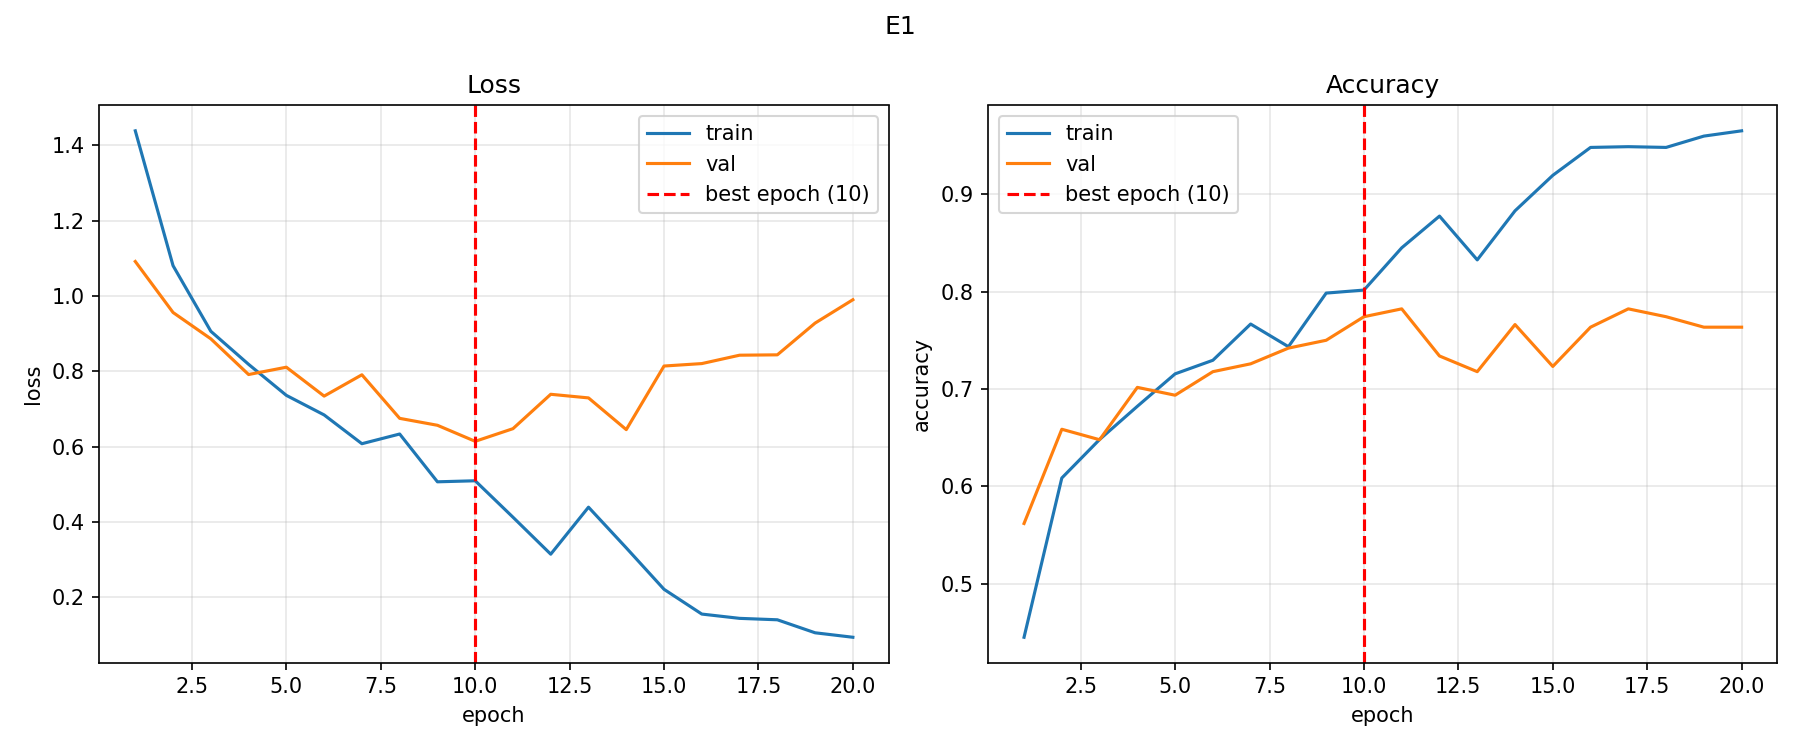
\includegraphics[width=\textwidth]{figuras/e1-curvas.png}
  \caption{E1: la pérdida de validación se desacopla pronto de la de entrenamiento.}
\end{subfigure}

\vspace{0.6em}
\begin{subfigure}[b]{0.72\textwidth}
  \centering
  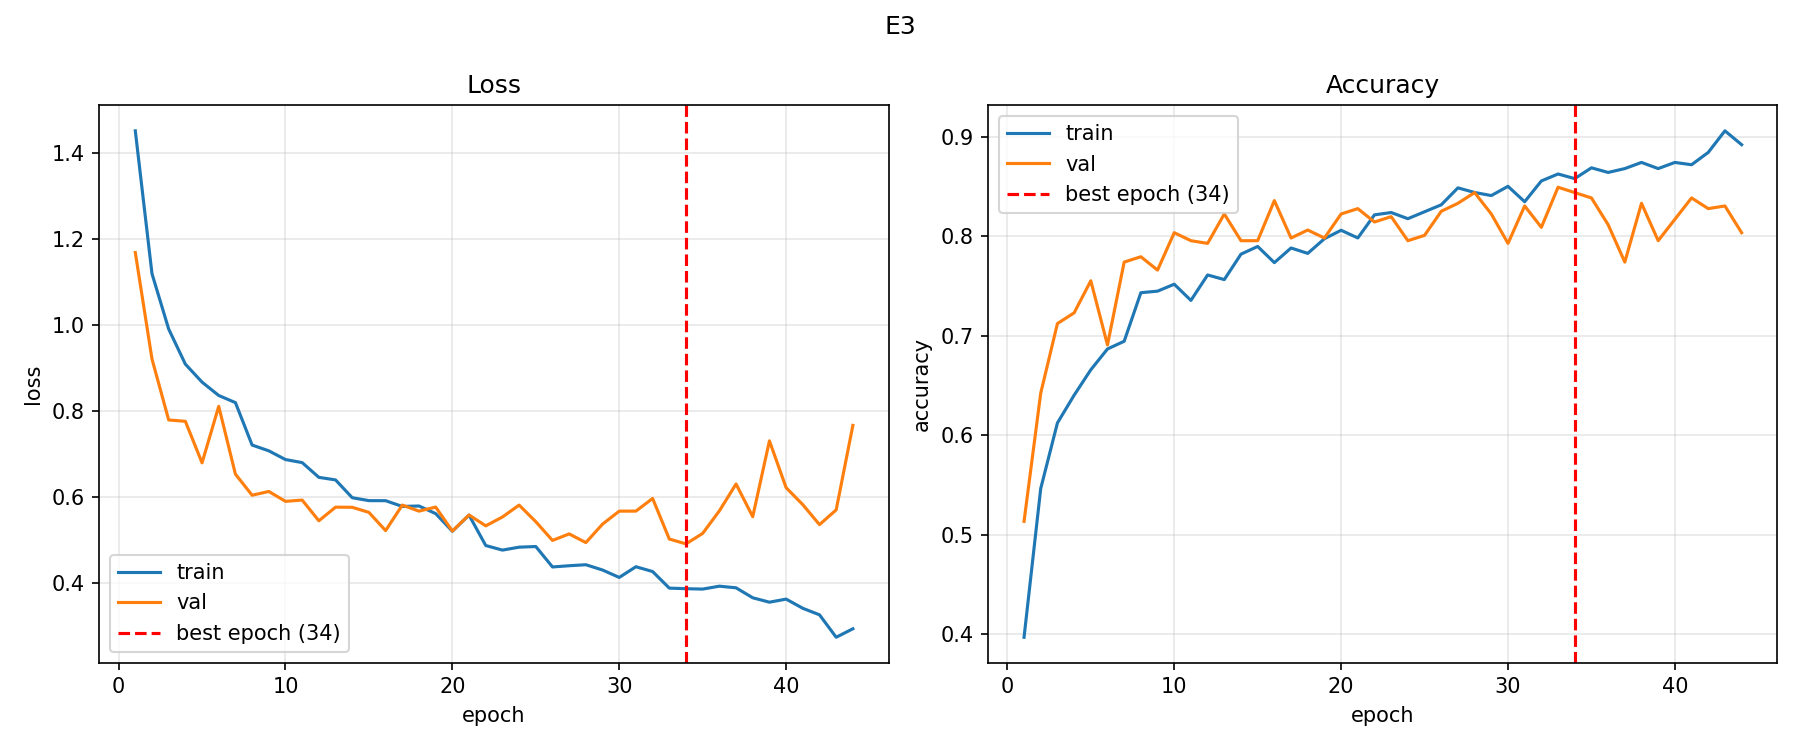
\includegraphics[width=\textwidth]{figuras/e3-curvas.png}
  \caption{E3: la augmentación y la normalización alargan la ventana productiva.}
\end{subfigure}
\caption{Curvas de pérdida y exactitud de entrenamiento y validación en la Fase~1.}
\label{fig:fase1}
\end{figure}

\paragraph{E1: el sobreajuste como límite.}
E1 reprodujo la referencia y obtuvo 0,7527 en test y 0,7742 en validación, lejos del objetivo. La causa no fue falta de capacidad: en la época óptima la brecha entre entrenamiento y validación era de solo 3,2 puntos. El problema fue la pendiente. Entre las épocas 11 y 21 la pérdida de entrenamiento cayó un $75\%$ mientras la de validación subió un $67\%$, y la brecha de exactitud llegó a 22,4 puntos. La parada temprana restauró los pesos de la mejor época y evitó entregar un modelo memorizado. La confusión se concentró en \emph{mountain} (exhaustividad 0,5161): ocho montañas se predijeron como \emph{buildings} y cinco como \emph{sea}. Es un solapamiento semántico, porque una montaña contiene árboles, si está sin nevar puede parecerse un edificio y si está nevada se puede confundir con un glaciar.

\paragraph{Nota de reproducibilidad.}
E1 se registró primero de forma ad hoc (mejor época 11, validación 0,7688, test 0,7742). Al pasar todas las pruebas por el ejecutor unificado se obtuvo mejor época 10, validación 0,7742 y test 0,7527. Esa diferencia de 1--2 puntos es el no-determinismo de CPU ya descrito; por eso las comparaciones usan el mismo ejecutor.

\paragraph{E2: la augmentación retrasa el sobreajuste.}
La augmentación desplazó la mejor época de la 10 a la 22 y el corte de la 20 a la 32. La pérdida de entrenamiento en la mejor época fue 0,5794 frente a 0,5098 en E1, mientras la de validación seguía bajando: exactamente el comportamiento que E1 había anticipado al atribuir el límite a la escasez de datos. La ganancia fue de $+5,64$ puntos en validación y $+3,22$ en test, insuficiente todavía para el $85\%$. \emph{Mountain} empeoró (exhaustividad 0,4516; diez montañas a \emph{buildings} y seis a \emph{sea}) porque el resto de clases mejoró y concentró el error en el caso difícil. La brecha validación--test se mantuvo en unos 4,6 puntos.

\paragraph{E3: la normalización cierra la brecha.}
La normalización con estadísticos de ImageNet llevó la mejor época a la 34 y el corte a la 44. El test subió a \textbf{0,8925} y la validación a 0,8441. La mejora grande se concentró en \emph{mountain}, cuya exhaustividad pasó de 0,4516 a 0,7419 (nueve aciertos más), y \emph{glacier} alcanzó precisión perfecta. La brecha validación--test se invirtió: el test quedó 4,8 puntos por encima de la validación. Ese cambio de signo entre dos ejecuciones consecutivas es la mejor evidencia de que las diferencias de test a esta escala son ruido y no deben leerse como mejoras exactas. Con todo, E3 es la mejor base: alcanza el objetivo y es más barata que E4.

\paragraph{E4: la resolución no aporta.}
Subir a $128\times128$ mejoró la validación 1,34 puntos (0,8575) pero bajó el test 5,92 (0,8333). Cuando validación y test se mueven en direcciones opuestas, lo más probable es ruido. Las clases que en teoría debían beneficiarse del detalle fino tampoco coincidieron: \emph{street} y \emph{mountain} subieron en validación, mientras \emph{buildings} y \emph{sea} bajaron en test. El coste, en cambio, es real: un $78\%$ más de píxeles por imagen y 917.504 parámetros adicionales en la primera capa totalmente conectada. Se elige E3, con un $42\%$ menos de parámetros.

\section{Fase 2: hiperparámetros (E5--E13)}

\subsection{Cribado de hiperparámetros}

La Tabla~\ref{tab:fase2} recoge las ocho configuraciones de la Fase~2, todas ellas partiendo de E3 y cambiando una sola variable.

\begin{table}[htbp]
\centering
\small
\caption{Cribado de hiperparámetros sobre E3. $\Delta$ val se mide en puntos porcentuales.}
\label{tab:fase2}
\begin{tabular}{llcccc}
\toprule
ID & Hiperparámetro & Cambio respecto a E3 & Mejor época & Val & $\Delta$ val \\
\midrule
E3 & referencia & --- & 34 & 0,8441 & --- \\
E5 & filtros convolucionales & 16-32-64 $\rightarrow$ 32-64-128 & 17 & 0,8199 & $-2{,}42$ \\
E6 & neuronas FC & 128 $\rightarrow$ 256 & 30 & 0,8360 & $-0{,}81$ \\
E7 & tasa de aprendizaje & $10^{-3}\rightarrow5\times10^{-4}$ & 28 & 0,8602 & $+1{,}61$ \\
E8 & tamaño de lote & 32 $\rightarrow$ 64 & 49 & 0,8602 & $+1{,}61$ \\
\textbf{E9} & activación & ReLU $\rightarrow$ ELU & 35 & \textbf{0,8817} & $\mathbf{+3{,}76}$ \\
E10 & capas convolucionales & 3 $\rightarrow$ 4 & 31 & 0,8306 & $-1{,}35$ \\
E11 & capas FC & 1 $\rightarrow$ 2 & 42 & 0,8522 & $+0{,}81$ \\
E12 & épocas y paciencia & 100 y 15 & 34 & 0,8441 & $0{,}00$ \\
\bottomrule
\end{tabular}
\end{table}

Los resultados permiten extraer cinco conclusiones:

\begin{itemize}
  \item \textbf{E9 (ELU) es el único resultado claro.} Mejora 3,76 puntos en validación y alcanza \textbf{0,9247} en test, el mejor de las doce configuraciones en ambos conjuntos. Mantiene la misma arquitectura y los mismos 1.245.862 parámetros que E3, de modo que la mejora procede solo de la activación.
  \item \textbf{Más capacidad perjudica.} Duplicar filtros (E5) cuesta 2,42 puntos de validación y duplicar neuronas (E6) cuesta 0,81. Con 1.290 imágenes de entrenamiento, añadir parámetros solo acentúa el sobreajuste.
  \item \textbf{Más profundidad convolutiva tampoco ayuda.} E10 cae 1,35 puntos en validación y 8,60 en test. Es la red más barata (860.966 parámetros, un $31\%$ menos), pero el cuarto \emph{pooling} deja la rejilla en $6\times6$ y se pierde información espacial.
  \item \textbf{El techo de épocas es inerte.} E12 devuelve exactamente E3: misma pérdida de validación (0,4908), misma mejor época (34) y mismo test. Quien decide es la parada temprana; el hiperparámetro real es la paciencia, no el techo.
  \item \textbf{E7, E8 y E11 son señal débil.} Sus ganancias (+1,61, +1,61 y +0,81) rozan o caen dentro del ruido, por lo que no se consideran ganancias probadas.
\end{itemize}

\subsection{Ensamblado E13}

E13 combinó los cambios que superaron 1,5 puntos sobre E3: ELU (E9), tasa de aprendizaje $5\times10^{-4}$ (E7) y lote 64 (E8), con techo 100 y paciencia 15 heredados de E12. La Tabla~\ref{tab:e13} lo compara con E9 y E3.

\begin{table}[htbp]
\centering
\small
\caption{Comparación del ensamblado E13 con la referencia E3 y la ganadora E9.}
\label{tab:e13}
\begin{tabular}{lccc}
\toprule
Métrica & E9 & E13 & E3 \\
\midrule
Mejor época & 35 & 29 & 34 \\
Pérdida de validación & 0,4456 & 0,4632 & 0,4908 \\
Exactitud de validación & \textbf{0,8817} & 0,8575 & 0,8441 \\
Exactitud de test & \textbf{0,9247} & 0,8280 & 0,8925 \\
Épocas ejecutadas & 45 & 44 & 44 \\
\bottomrule
\end{tabular}
\end{table}

La regla predefinida decide: \textbf{se queda E9}. E13 alcanza 0,8575 en validación, 2,42 puntos por debajo de E9 y por debajo de la barra de 0,90 fijada antes de ejecutar. En test la caída es mayor, 9,67 puntos (0,9247 $\rightarrow$ 0,8280). Los dos conjuntos coinciden, así que no hay ambigüedad: E7 y E8 no aportan nada sobre E9 y, de hecho, lo degradan.

La predicción sobre el techo resultó errónea. Se esperaba que combinar la mitad de tasa de aprendizaje con el doble de lote ralentizara tanto el entrenamiento que E13 agotara las 100 épocas. En realidad la parada temprana cortó en la 44 y el mejor modelo quedó en la 29, antes incluso que el 35 de E9: ELU acelera la convergencia lo suficiente para compensar con creces la tasa reducida. La lectura más directa del empeoramiento es que E7 y E8 eran ruido favorable —subían validación y bajaban test— y que sumar ruido a una buena configuración solo la degrada.

E9 queda como la mejor configuración desde cero: 0,9247 en test, los mismos parámetros que E3 y el mismo coste por época. Es la única que gana a E3 simultáneamente en validación y en test, y supera holgadamente el objetivo. Las Figuras~\ref{fig:e9curvas} y~\ref{fig:e9confusion} muestran sus curvas y su matriz de confusión.

\begin{figure}[htbp]
\centering
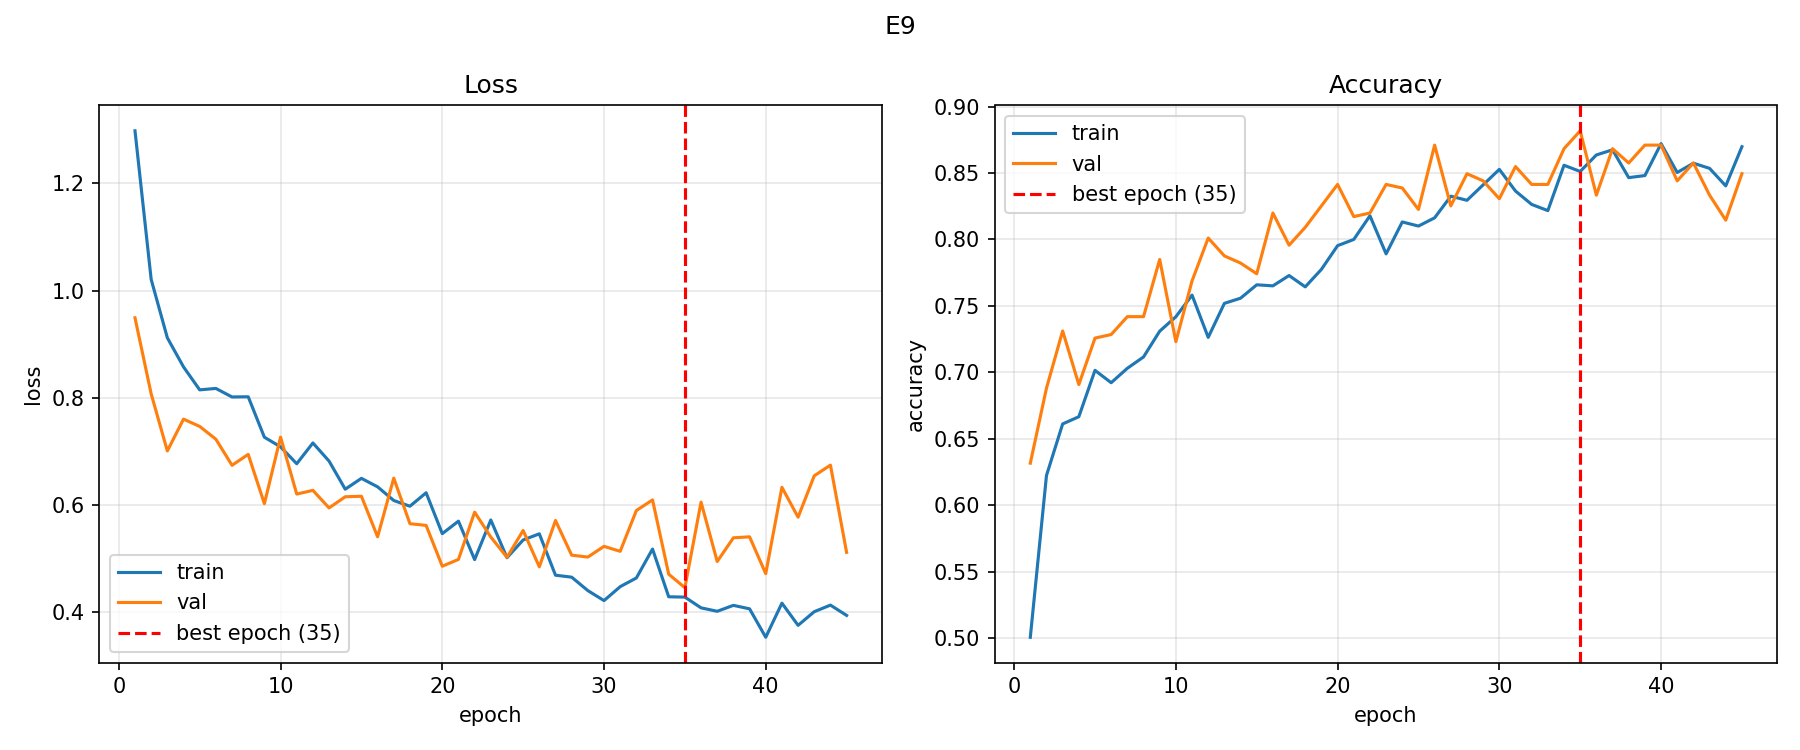
\includegraphics[width=0.62\textwidth]{figuras/e9-curvas.png}
\caption{Curvas de E9. La ventana productiva llega hasta la época 35 y la validación acompaña al entrenamiento durante más tiempo que en E1.}
\label{fig:e9curvas}
\end{figure}

\begin{figure}[htbp]
\centering
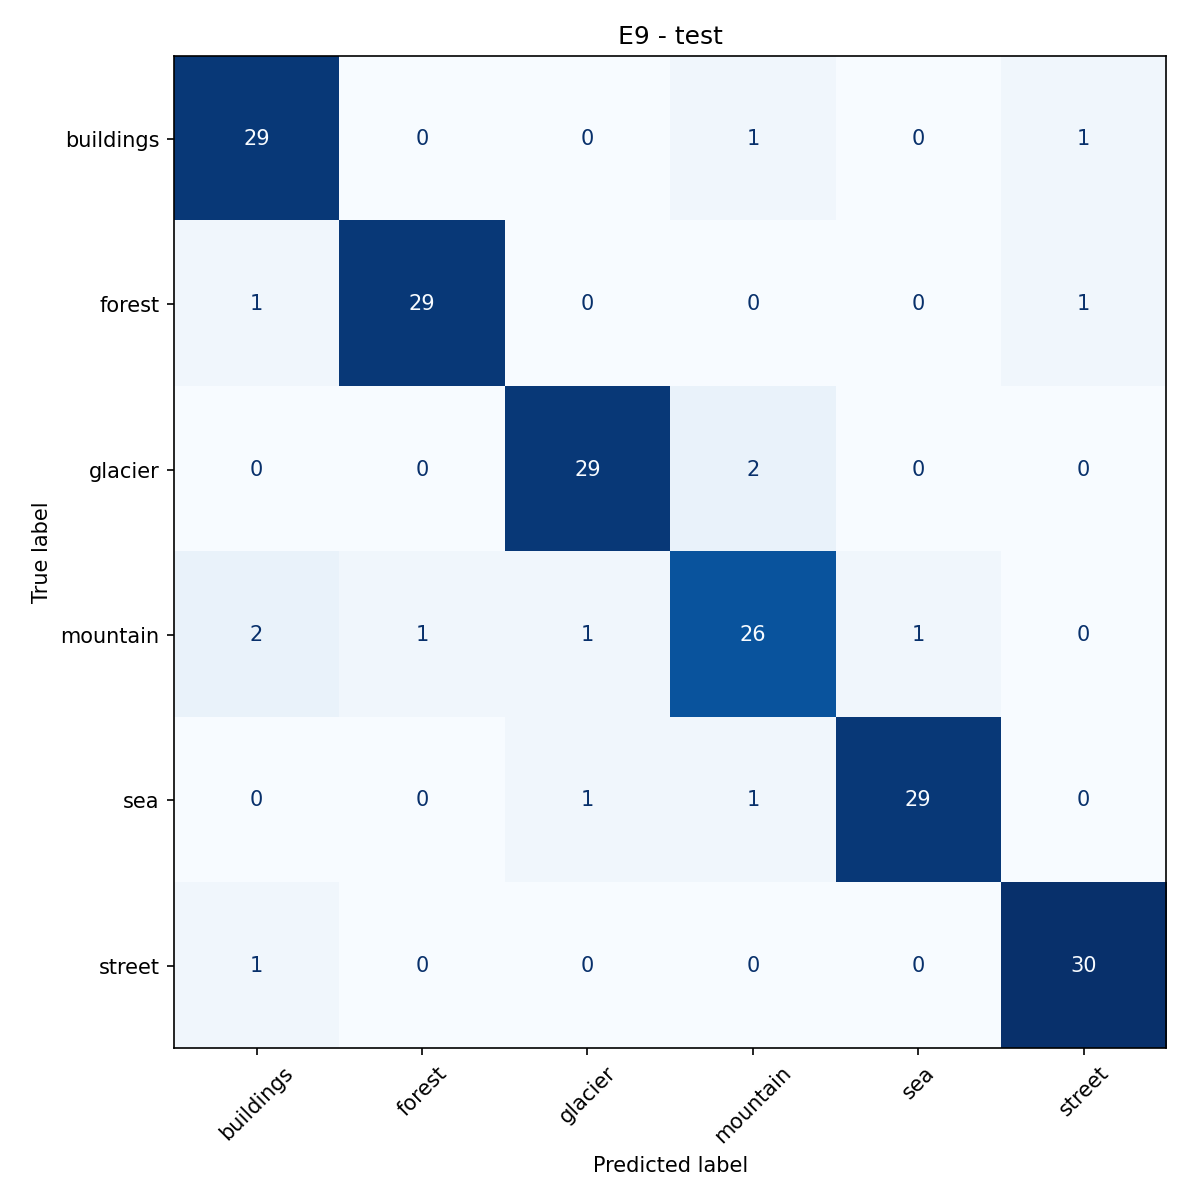
\includegraphics[width=0.42\textwidth]{figuras/e9-confusion-test.png}
\caption{Matriz de confusión de E9 en test. Los errores se concentran en \emph{mountain}, \emph{glacier} y \emph{sea}.}
\label{fig:e9confusion}
\end{figure}

\section{Transfer learning (E14 y E15)}

\subsection{Motivación y protocolo}

El diagnóstico de E1 y E2 fue que el límite no era la capacidad sino la escasez de datos: la \texttt{ConvNet} con 1,25 millones de parámetros sobre 1.290 imágenes entraba pronto en sobreajuste. El transfer learning ataca directamente ese problema: no hay que aprender las características, sino reutilizarlas. ResNet18, entrenada sobre ImageNet con 1,28 millones de imágenes y 1.000 clases, ya distingue texturas, bordes y formas; basta con sustituir la cabeza y entrenar solo esa parte.

No se transfiere el modelo de E9. E9 es el rival al que batir, no el punto de partida. Lo que se transfiere es el protocolo: el reparto de datos y la semilla 42, la normalización y la augmentación de E3, Adam con tasa $10^{-3}$, la activación ELU y la parada temprana con techo 50 y paciencia 10. Cambian solo el modelo y su resolución de entrada, dos decisiones inseparables de adoptar transfer learning.

\subsection{Correcciones al ejemplo de referencia}

La estructura se tomó del cuaderno de transfer learning del ejemplo, pero ese cuaderno apunta a Colab y contiene cuatro defectos que aquí se corrigieron: (i) no normaliza la entrada, aunque los pesos de ImageNet esperan esa normalización; (ii) el bucle de validación solo registra el último lote de cada época, de modo que su pérdida no es la media del conjunto; (iii) declara listas de exactitud que nunca utiliza; y (iv) no incorpora parada temprana, requisito obligatorio de la práctica. Además, la cabeza usa ELU en lugar de ReLU para que E9 y E14 sean comparables manteniendo la activación constante.

\subsection{Resultados}

La Tabla~\ref{tab:tl} compara E14 y E15 con E9.

\begin{table}[htbp]
\centering
\small
\caption{Resultados del transfer learning frente a la mejor red desde cero.}
\label{tab:tl}
\begin{tabular}{lccc}
\toprule
Métrica & E9 & \textbf{E14} & E15 \\
\midrule
Mejor época & 35 & 21 & 7 \\
Pérdida de validación & 0,4456 & 0,1098 & \textbf{0,0121} \\
Exactitud de validación & 0,8817 & 0,9543 & \textbf{0,9946} \\
Exactitud de test & 0,9247 & \textbf{0,9785} & 0,9731 \\
F1 \emph{macro} en test & --- & \textbf{0,9785} & 0,9732 \\
Épocas ejecutadas & 45 & 31 & 17 \\
Parámetros entrenables & 1.245.862 & \textbf{66.438} & 8.460.166 \\
\bottomrule
\end{tabular}
\end{table}

El transfer learning gana a E9 en ambos conjuntos y con un margen mucho mayor que cualquier diferencia entre hiperparámetros. E14 suma 7,26 puntos en validación (0,8817 $\rightarrow$ 0,9543) y 5,38 en test (0,9247 $\rightarrow$ 0,9785), y lo hace con \textbf{19 veces menos parámetros entrenables}. La ganancia de validación duplica el margen de error de 372 imágenes, y el test se mueve en la misma dirección con una magnitud parecida. La conclusión es coherente con el diagnóstico de E1: lo que faltaban eran datos, no capacidad.

E14 y E15 son indistinguibles en test: la diferencia es de una imagen. Con 186 imágenes, E14 se equivoca 4 veces y E15 5. Esa diferencia está muy por debajo del margen de $\pm5$ puntos y no permite rankear. Por la regla predefinida, el ranking se hace por validación, donde E15 obtiene 0,9946 (370 de 372, solo dos errores) frente a 0,9543 de E14. Sin embargo, la validación de E15 está inflada, y hay dos pruebas.

La primera es que la brecha validación--test cambia de signo: en E14 el test supera a la validación en 2,42 puntos; en E15 queda 2,15 puntos por debajo. La segunda es la relación entre pérdidas: en su mejor época E15 registra una pérdida de entrenamiento de 0,1171 y una de validación de 0,0121, diez veces menor. Que la validación supere al entrenamiento es esperable, porque este lleva augmentación y \emph{dropout} activos, pero esa magnitud es extrema. El mecanismo es sobreajuste a la validación por selección: la parada temprana elige la mejor época mirando \texttt{val\_loss}, y E15 completó 17 rondas de selección sobre las mismas 372 imágenes con 8,46 millones de parámetros disponibles. La pérdida de validación nunca subió de forma sostenida y el corte llegó muy por debajo del techo de 50.

El punto ciego persistente es la confusión \emph{glacier} $\rightarrow$ \emph{mountain}. Aparece en el cuarto modelo consecutivo: los dos únicos errores de E15 en validación fueron hacia \emph{mountain}, y E14 acumula siete en validación y dos en test. Que persista con características de ImageNet, entrenadas con un millón de imágenes, indica que no es un problema de capacidad ni de datos, sino de solapamiento real entre ambas categorías.

Se adopta \textbf{E14 como referencia}: empata en test con E15 con 19 veces menos parámetros entrenables y su validación resultó pesimista, por lo que es la estimación más honesta de generalización. Descongelar \texttt{layer4} añade 8,39 millones de parámetros sin una ganancia demostrable en el conjunto no visto. Las Figuras~\ref{fig:e14confusion} y~\ref{fig:e15confusion} muestran las matrices de confusión.

\begin{figure}[htbp]
\centering
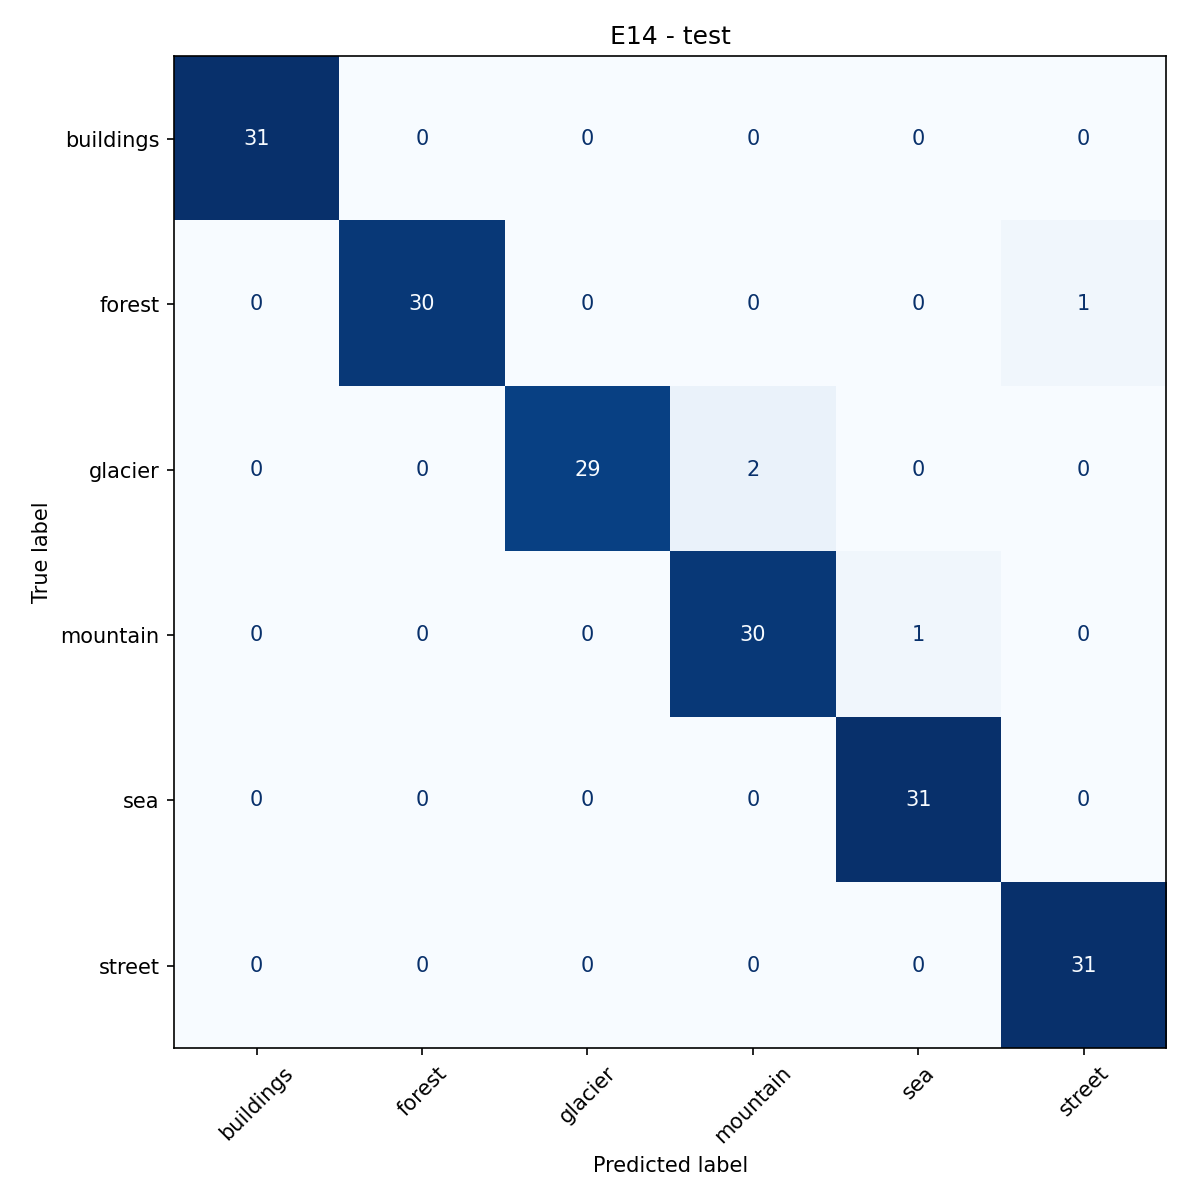
\includegraphics[width=0.42\textwidth]{figuras/e14-confusion-test.png}
\caption{Matriz de confusión de E14 en test: cuatro errores sobre 186 imágenes.}
\label{fig:e14confusion}
\end{figure}

\begin{figure}[htbp]
\centering
\begin{subfigure}[b]{0.40\textwidth}
  \centering
  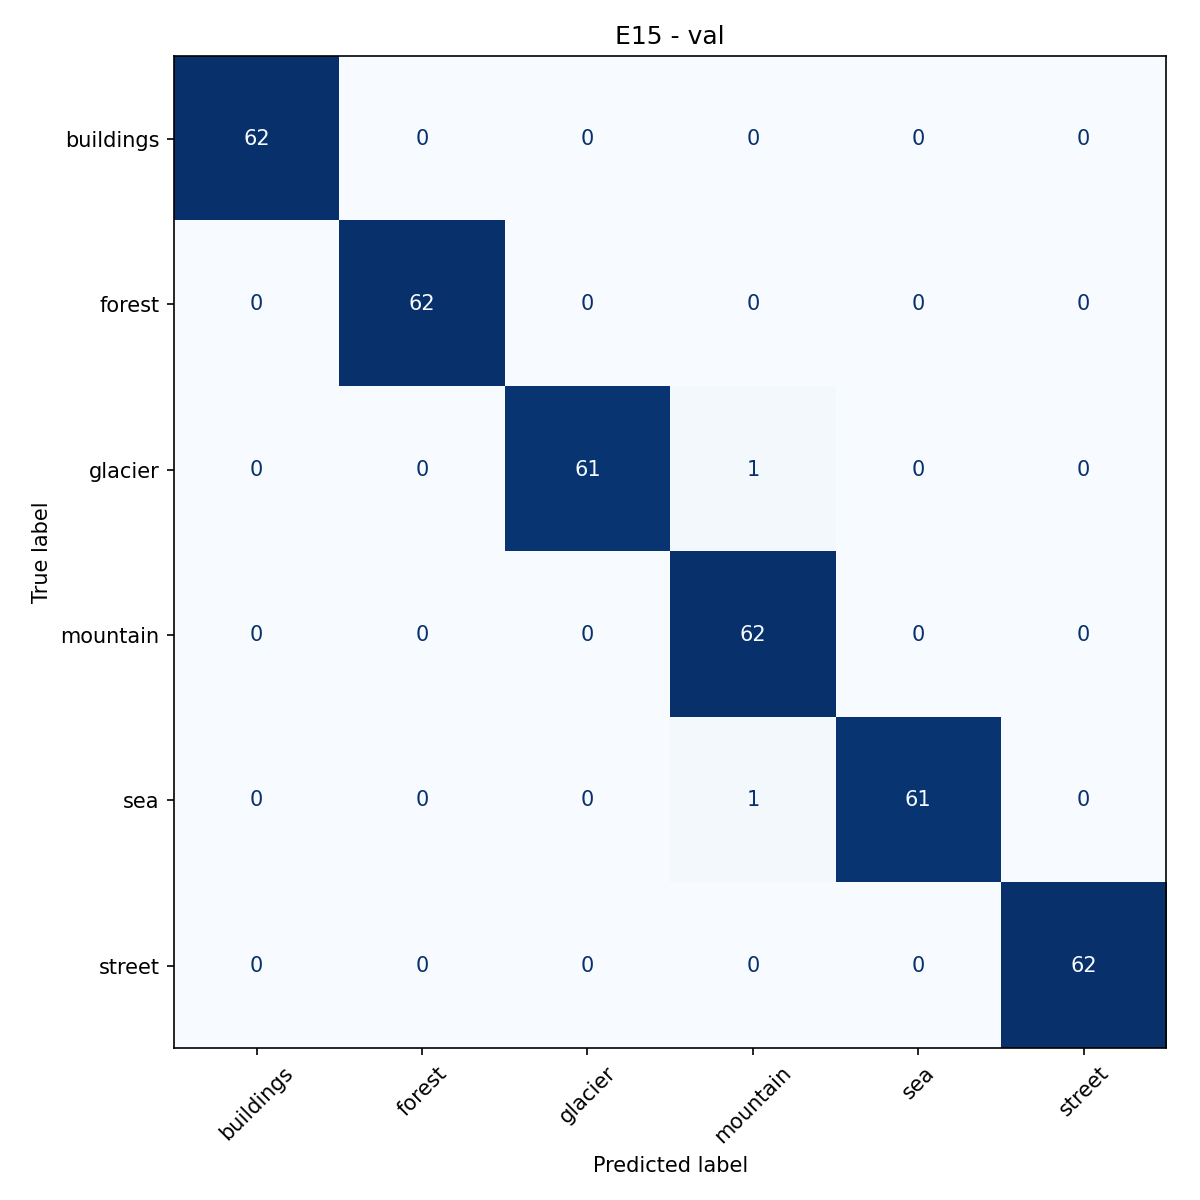
\includegraphics[width=\textwidth]{figuras/e15-confusion-val.png}
  \caption{Validación: 2 errores.}
\end{subfigure}
\hfill
\begin{subfigure}[b]{0.40\textwidth}
  \centering
  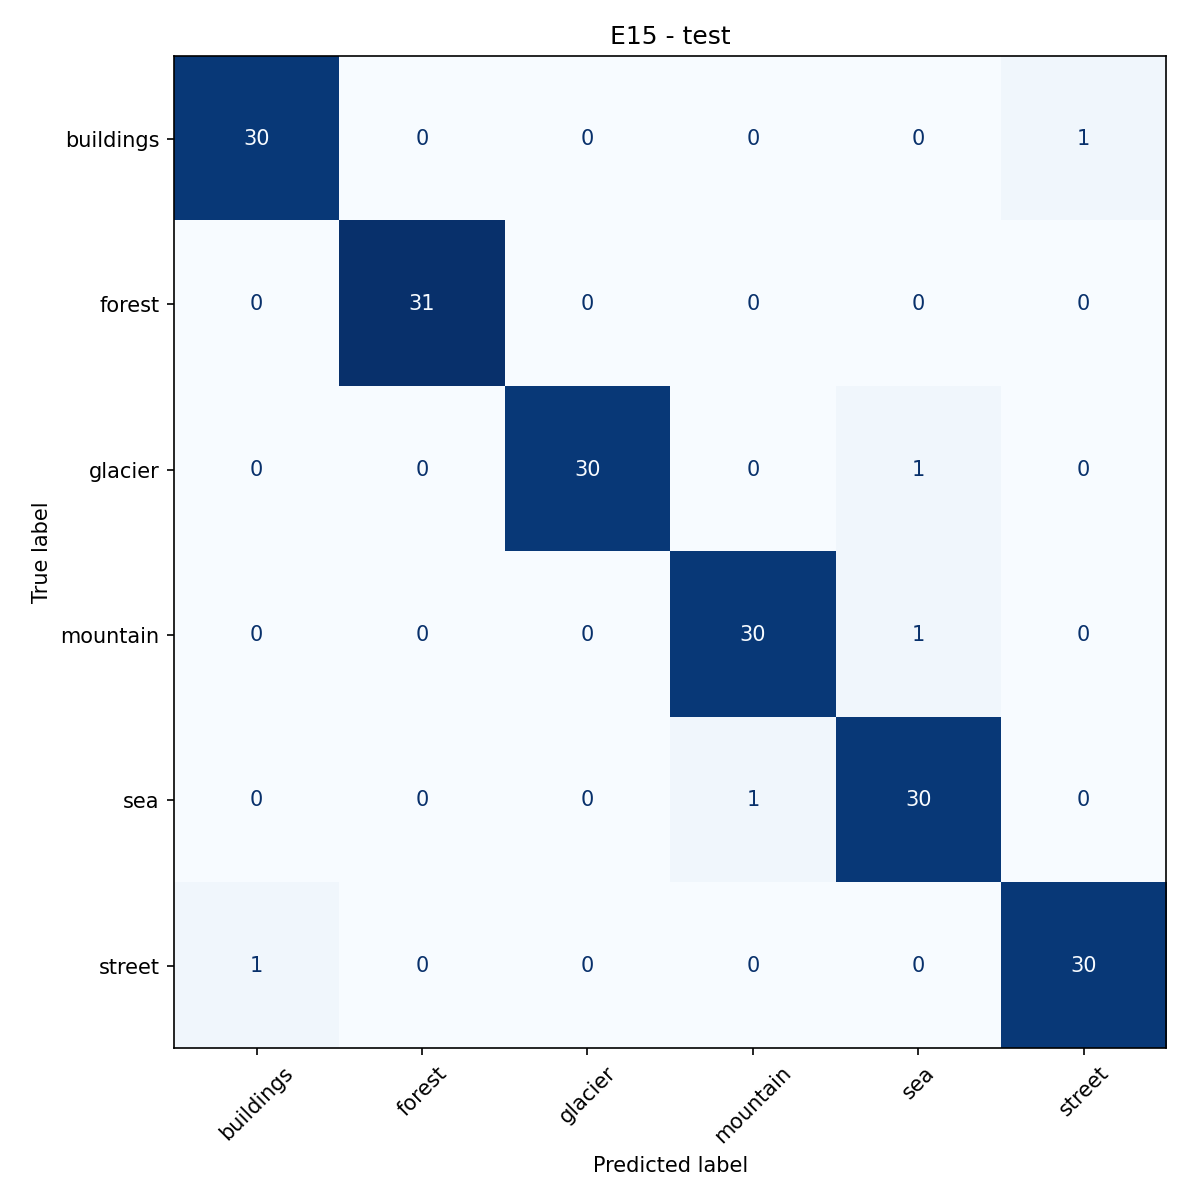
\includegraphics[width=\textwidth]{figuras/e15-confusion-test.png}
  \caption{Test: 5 errores.}
\end{subfigure}
\caption{Matrices de confusión de E15. La validación, aparentemente casi perfecta, está inflada por la selección de la mejor época.}
\label{fig:e15confusion}
\end{figure}

\section{Discusión}

La Figura~\ref{fig:comparativa} reúne la exactitud de validación y test de las quince configuraciones. A partir de ella y de los resultados anteriores se pueden extraer varias lecciones.

\begin{figure}[htbp]
\centering
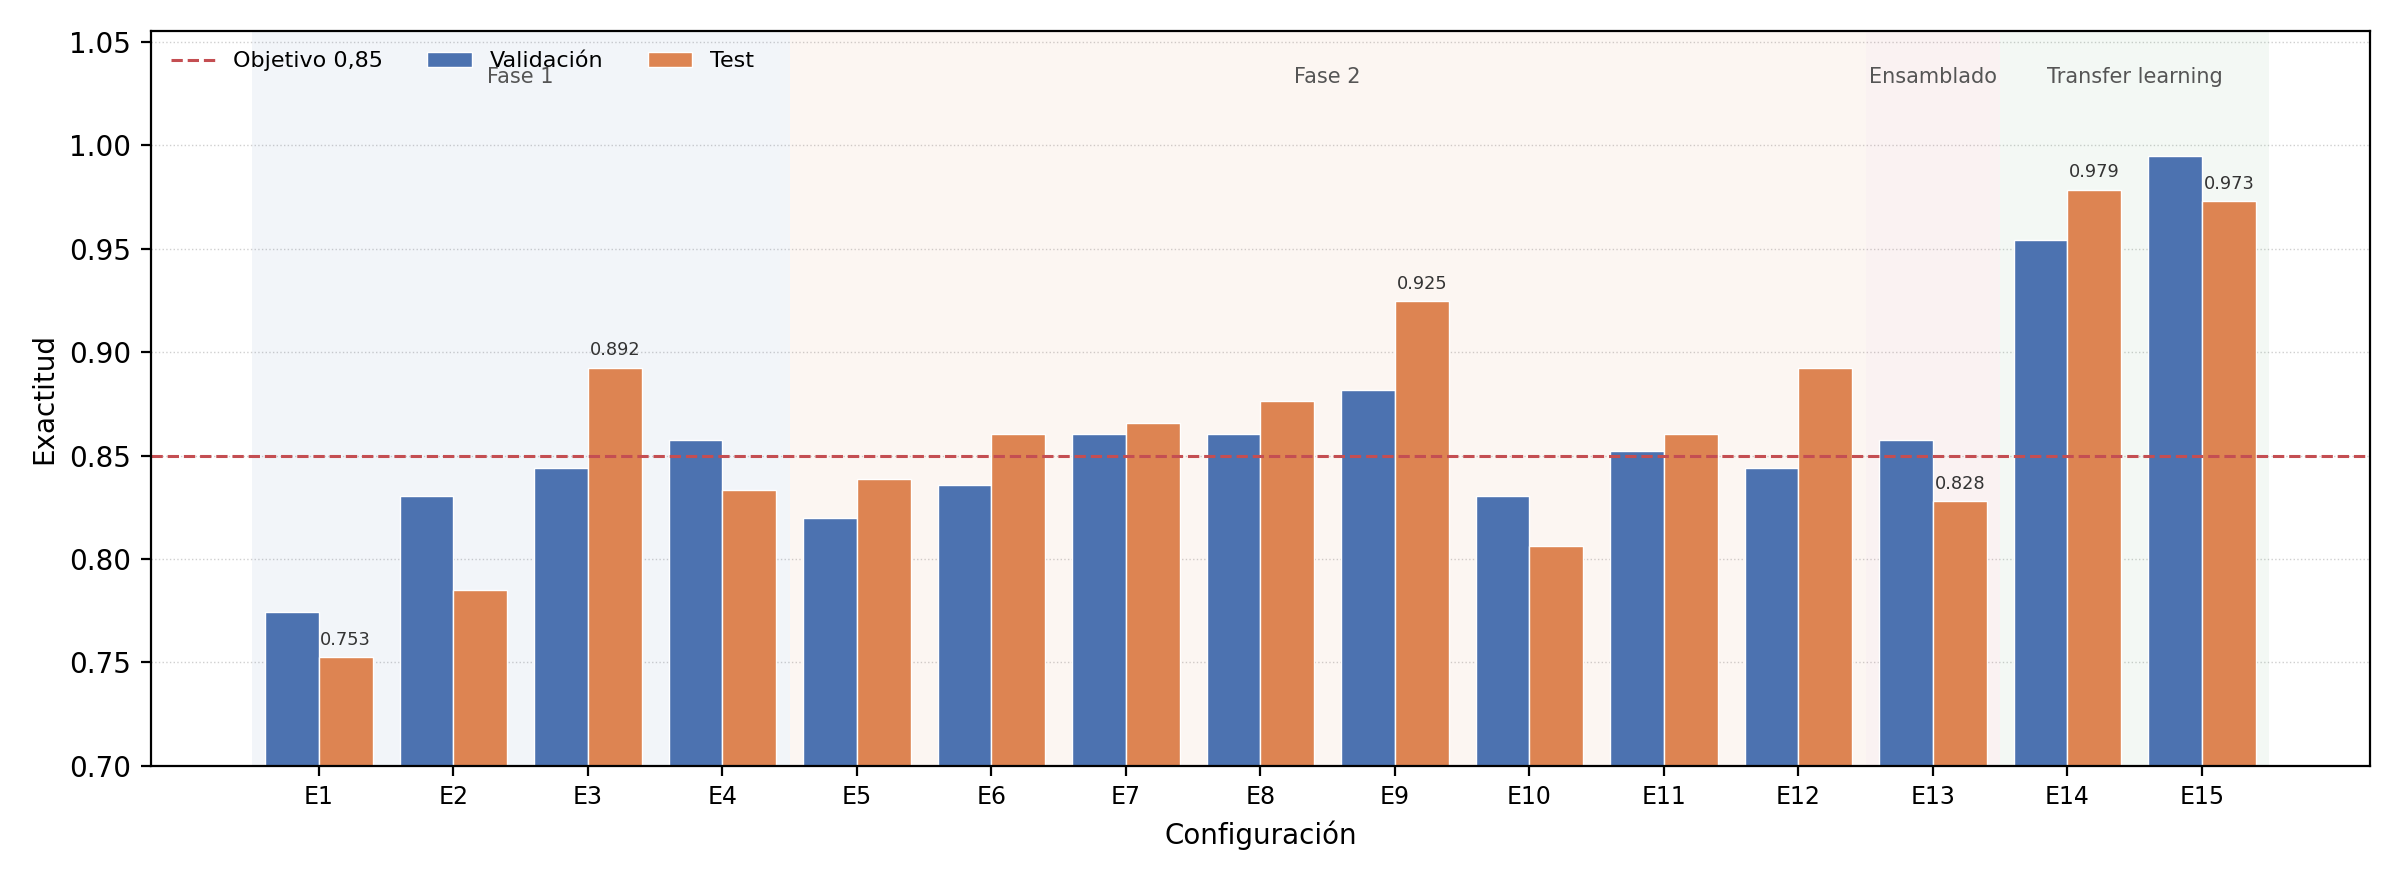
\includegraphics[width=0.95\textwidth]{figuras/comparativa.png}
\caption{Exactitud de validación y test de las quince configuraciones, agrupadas por fase. La línea discontinua marca el objetivo del $85\%$.}
\label{fig:comparativa}
\end{figure}

\paragraph{Datos, no capacidad.}
E1 ya lo insinuaba: en su mejor época apenas había brecha entrenamiento--validación y, sin embargo, el modelo se saturaba. Las pruebas posteriores lo confirman desde tres ángulos. Aumentar la augmentación (E2) retrasa el sobreajuste y mejora; aumentar filtros, neuronas o profundidad (E5, E6, E10) empeora; y reutilizar características de ImageNet (E14) da el salto mayor con 19 veces menos parámetros entrenables. El cuello de botella era la cantidad y la diversidad de los datos, no la capacidad del modelo.

\paragraph{El preprocesado pesa más que los hiperparámetros.}
En la Fase~1, la normalización y la augmentación produjeron la mayor parte de la mejora desde cero. En la Fase~2, de ocho hiperparámetros solo la activación ELU superó el ruido de forma clara. Esto no significa que los hiperparámetros sean irrelevantes, sino que su efecto depende del preprocesado: buscar épocas o tasa de aprendizaje sobre E1 habría llevado a conclusiones falsas, porque su ventana productiva era un artefacto de la falta de regularización.

\paragraph{ELU como única mejora clara.}
E9 mejora 3,76 puntos en validación y 4,22 en test respecto a E3 sin añadir un solo parámetro. La explicación plausible es que su saturación suave en valores negativos facilita la optimización frente a ReLU, pero el experimento no permite aislar el mecanismo; lo que sí establece es que el cambio es robusto y barato. E13 demuestra que combinarlo con otros cambios que parecían favorables no funciona: las interacciones importan y el cribado univariante no las detecta.

\paragraph{Transfer learning: congelar basta.}
E14 supera a E9 con un margen que duplica el ruido y con una fracción mínima de parámetros entrenables. Descongelar el último bloque (E15) no mejora el test y, además, infla la validación por selección. Para un conjunto de este tamaño, congelar el backbone entero es la opción más eficiente y la más honesta metodológicamente.

\paragraph{Confusión semántica irreducible.}
\emph{Mountain} y \emph{glacier} se solapan de forma persistente en todos los modelos, incluido el transfer learning. Una montaña nevada es, visualmente, un glaciar con roca; una ladera con nieve puede etiquetarse de cualquiera de las dos formas. Este límite no se resuelve con más capacidad ni con más épocas, sino con datos mejor etiquetados, información adicional o un enfoque de segmentación. Es un buen recordatorio de que el techo de un clasificador también lo pone la definición de las clases.

\paragraph{Ruido de evaluación y sobreajuste a validación.}
Las diferencias de test entre configuraciones cercanas cambian de signo con frecuencia (E3 frente a E4, E9 frente a E13, E14 frente a E15). Con 186 imágenes, una sola predicción mueve 0,54 puntos. Por eso el ranking se hizo por validación y por eso se auditó la brecha validación--test. E15 muestra el riesgo complementario: cuando se selecciona la mejor época sobre el mismo conjunto que se usa para rankear, la validación deja de ser una estimación insesgada. Fijar las reglas antes de ejecutar y reservar el test para el final son las dos salvaguardas que se aplicaron.

\paragraph{Reproducibilidad.}
El ejecutor único, la semilla fija y las particiones congeladas hacen que el pipeline sea reproducible en lo grueso, pero no bit a bit: las reducciones multihilo de CPU introducen 1--2 puntos de variación. Documentar esa variación es parte del resultado, porque sin ella se correría el riesgo de interpretar como mejora lo que es ruido.

\section{Conclusiones}

El objetivo de alcanzar al menos un $85\%$ de exactitud en test se cumple con margen. La mejor configuración desde cero, E9, obtiene \textbf{0,9247} con 1.245.862 parámetros y activación ELU. La mejor configuración global, E14, obtiene \textbf{0,9785} con una ResNet18 preentrenada y solo 66.438 parámetros entrenables. En total se documentan quince configuraciones que cubren los siete hiperparámetros del enunciado, el preprocesado, un ensamblado y dos variantes de transfer learning.

Las lecciones principales son tres. Primera, el límite del problema era la escasez de datos, no la capacidad: por eso la augmentación y el transfer learning aportaron más que cualquier cambio arquitectónico. Segunda, conviene fijar el preprocesado antes de buscar hiperparámetros, porque la ventana de entrenamiento y el efecto de cada hiperparámetro dependen de él. Tercera, con conjuntos de test pequeños es imprescindible separar selección de evaluación y fijar las reglas antes de ver los resultados; de lo contrario, el ruido se confunde con mejora.

El trabajo tiene limitaciones claras: un único subconjunto curado, una sola semilla, un solo equipo de CPU y un test de 186 imágenes. Como trabajo futuro resultaría natural repetir la comparación con validación cruzada y varias semillas, ampliar el conjunto de entrenamiento, probar otros backbones y aplicar técnicas de interpretabilidad para verificar si la confusión \emph{mountain}--\emph{glacier} se corresponde con regiones realmente ambiguas de la imagen.

\bibliography{referencias}

\end{document}
